\documentclass[a4paper,10pt]{scrreprt}
\usepackage[utf8]{inputenc}

\usepackage{graphicx} % Required for including pictures
\usepackage{listings}
\usepackage{float} % Allows putting an [H] in \begin{figure} to specify the exact location of the figure
\usepackage{wrapfig} % Allows in-line images such as the example fish picture
\usepackage{color}
\linespread{1.2} % Line spacing
\setcounter{tocdepth}{4}

\lstset{frame=tb,
  language=perl,
  aboveskip=3mm,
  belowskip=3mm,
  showstringspaces=false,
  columns=flexible,
  basicstyle={\small\ttfamily},
  numbers=none,
  breaklines=true,
  breakatwhitespace=true,
  breaklines=true,
  frame=none
}


% Title Page
\title{DOME\\A rest-inspired engine for DPM}
\author{}

\subtitle{DMLite 0.8.0}

\begin{document}
\maketitle

\begin{abstract}


The DPM (Disk Pool Manager) project is the most widely deployed solution for storage of large
data repositories on Grid sites, and is completing the most important upgrade in its history,
with the aim of bringing important new features, performance and easier long term maintainability.
Work has been done to make the so-called "legacy stack" optional, and substitute it with
an advanced implementation that is based on the fastCGI and RESTful technologies.
Beside the obvious gain in making optional several legacy components that are difficult
to maintain, this step brings important features together with performance enhancements.
Among the most important features we can cite the simplification of the configuration,
the possibility of working in a totally SRM-free mode, the implementation of quotas,
free/used space on directories, and the implementation of volatile pools that
can pull files from external sources, which can be used to deploy simple data caches.

Moreover, the communication with the new core, called DOME (Disk Operations Management Engine)
now happens through secure HTTPS channels through an extensively documented,
industry-compliant protocol.

\end{abstract}



\newpage % Begins the essay on a new page instead of on the same page as the table of contents


%----------------------------------------------------------------------------------------
%	TABLE OF CONTENTS
%----------------------------------------------------------------------------------------

\tableofcontents % Include a table of contents

\newpage % Begins the essay on a new page instead of on the same page as the table of contents



\chapter{Dome}

DOME (Disk operations Management Engine) is a robust, high performance server that manages the operations of a DPM cluster. DOME is built on the FastCGI technology,
and uses HTTP and JSON to communicate with clients.
This initiative aims at augmenting the Disk Pool Manager (DPM) system so that its core coordination functions and inter-cluster communication paths are
implemented through open components, and following contemporary development approaches headed to performance, scalability and maintainability. Among our goals we cite:

\begin{itemize}
 \item Making optional all the so-called legacy components that are provided by the \textit{lcg-dm} code tree, namely \textit{libshift}, \textit{rfiod},
 \textit{dpm(daemon)}, \textit{dpnsdaemon}, \textit{CSec} and others.
 \item provide a software infrastructure where adding new coordination features is easier than with \textit{lcg-dm}
 \item provide full support for asynchronous calculation of file checksums of multiple types
 \item provide support for checking the consistence of replicas through their checksums
 \item provide structure, hooks and callouts that allow the usage of DPM as a fast and large \textit{file cache}
 \item having a unified configuration file that is readable and synthetic, as opposed to the \textit{lcg-dm} approach of having several configuration
 files here and there, all with differently over-simplified syntax rules (or no syntax at all, e.g. \textit{/etc/NSCONFIG})
\end{itemize}

The DOME component has the shape of a \textit{fastCGI} daemon, and has to be triggered by the Apache instances running in the DPM head node and
in all the DPM disk servers. A configuration option defines whether it is running as head node or disk server.

For simplicity of expression, in this document we may refer to these modalities as two different components, named \textit{DOMEhead} and \textit{DOMEdisk}.
In practice, these refer to the same component which has been given a different command-line flag to enable/disable a different command set,
implemented in the same software skeleton.\\

DOME is primarily a service provider for the \textit{dmlite} framework, through the dmlite plugin called DOMEAdapter.\\

\section{DOME: Main features}
DOME has two modalities: headnode and disknode, which respectively represent evolutions of the \textit{dpm} daemon and of \textit{rfiod}, together with \textit{libshift} and \textit{Csec}.
The functionalities are roughly as follows:
\begin{itemize}
 \item headnode: general coordination function
 \subitem spreads load (PUT, GET, checksums) towards the available disk nodes
 \subitem keeps an in memory status of the DPM disk/pool topology with disk sizes and free space
 \subitem keeps an in memory status of the ongoing asynchronous checksum calculations
 \subitem keeps an in memory status of the ongoing asynchronous file callouts
 \subitem queues and dispatches to disk nodes the requests for asynchronous checksum calculations that have to be delayed for load balancing reasons
 \subitem queues and dispatches to disk nodes the requests for asynchronous file callouts that have to be delayed for load balancing reasons

 \item disknode: local disk and space-related services
 \subitem Allows to \textit{stat} individual physical files and directories
 \subitem Allows to \textit{statfs} filesystems to get used and free space
 \subitem Allows the local submission of checksum calculations
 \subitem Allows the local submission of file callouts
\end{itemize}

The historical tunnelling feature provided by the \textit{rfio} infrastructure (and used by gridftp in some boundary scenarios)
is implemented by DOMEAdapter directly on the top of HTTP, hence namely it does not use the DOME server.\\


The main difference from the legacy components is that DOME does not apply authorization again for individual user file
access, as this task is already accomplished by the dmlite frontends. DOME only checks that the sender of a request is authorized to
send requests, in a way that is similar to the libshift "root mode". DOME applies strong, industry standard authentication protocols to this task.\\
Authentication in DOME is zero-config for the regular cases (one head node and multiple disk servers), and flexible enough
to add arbitrary identities that will be allowed to send commands to it.\\

\textbf{DOME is protocol-agnostic. Its concepts of logical file name and physical file name are not linked to a particular data/metadata transfer protocol.
DOME manages paths and filenames, not URLs. URLs can be constructed by the DPM frontends starting from the pfn or lfn information given by DOME.}


\subsection{From spacetokens to quota tokens}
Historically, DPM does space accounting through a set of individual named space reservations, kept in the DB in the head node, and associated to pools.\\
Semantically, space reservations are named reservations of a part of the space of a disk pool. Requests to write a replica specify a pool
that has to host the replica, hence ultimately the replica will be subject to the space reservations.\\

One of the weakest points in this schema is that the writer has to know technical details of the destination storage, to be able to write
and be properly accounted for.\\

Another historical weak point is that calculating good numbers for the space occupancies can be a challenging exercise, especially if the structure of the pools
has been modified in the years.\\
The development direction of DOME is to evolve this mechanism towards \textit{subdirectory\-based space accounting}, instead than pool-based.\\

In subdirectory-based space accounting, every subdirectory at less than N levels from the root is kept updated with the total size of the replicas
of files that reside in that directory subtree.\\

This \textit{subdirectory size} together with the information on free/used space in the pools associated to these subdirectory tree
can then be used to compute the needed space occupancy numbers.

DOME uses the records describing spacetokens that are kept in the head node DB, with minimal modification. Their meaning is slightly changed,
into semantically representing a quota on one and only one directory subtree. From this point on, we will refer to them as \textit{quotatokens},
whose behavior is similar to that of an old spacetoken associated to a directory.\\

A \textit{quotatoken} attached to a directory subtree \textbf{overrides others that may be attached to its parents}.\\
If a directory content (counting all the replicas) exceeds the quota spacified by the quotatoken that influences it,
then new PUT requests on that dir will be denied.\\

As a summary, the meaning of a quotatoken specifying a quota of N on poolX, associated to directory "/dir1" is \textit{give poolX as
space for hosting the files that will be written into \/dir1. Do not allow more than N terabytes to be hosted there}.\\

\subsection{Pools and filesystems}
A pool is a logical group of mount points in individual disk servers that are used to store replicas.\\

DOME uses the same concept of Pool than the historical DPM, hence the "Pool management" functionalities
of the legacy lcg-dm components continue to work mostly as they were.\\

A Pool can be associated to a directory subtree by creating suitable quotatokens that describe the individual associations.\\

A Pool assigned to a subtree acts as a sort of "replication domain". Replicas of files belonging to that subtree
are stored in filesystems belonging to this pool. Multiple replicas are spread through different file systems.\\

We would like to emphasize that only one pool can be assigned to the same directory subtree (e.g. /dpm/cern/ch/home/dteam/scratch).
Writes into this subtree will be space-balanced between all the filesystems composing the pool assigned to it. A pool instead can be associated
to any number of quotatokens (and hence, directories).\\

\subsection{Open checksumming}
DOME supports requests for checksums of arbitrary kind. It can:\\

\begin{itemize}
 \item return the corresponding checksum that is stored in the name space
 \item choose an appropriate replica of the file and tell to the disk node managing it to calculate its checksum
 \item force the recalculation of the checksum and store it into the name space
\end{itemize}

The checksum calculation request may be queued in the head node, in memory. The architecture is designed to be self-healing in the case the checksum
calculations do not end correctly, or some machines are restarted.





\section{Tech}

The architecture of DOME is expandable, through the usage of an open, human-readable protocol (JSON) and through proper design.\\


\subsection{Architecture}
Figure \ref{figdomedisk} shows the main components of DOME that are in action in a disk server.\\
Requests come through Apache already authenticated and referring to the two possible paths that
refer either to the filesystems or to the dome command path which starts with \lstinline{/domedisk}.
Another detail that characterizes a disk server for DOME is the ability to execute tasks like checksum calculations
and file pulls from external sources. These tasks, following a logic that is based on time, report their status
to the head node, which uses this information to keep its queues updated.\\
 
\begin{figure}
\begin{center}
 \includegraphics[width=10cm,keepaspectratio=true,angle=-90,origin=c]{./pics/domepics_disk.eps}
 % domepics_disk.ps: 0x0 pixel, 300dpi, 0.00x0.00 cm, bb=
 \caption{Simplified diagram of DOME in a disk node}
 \label{figdomedisk}
\end{center}
\end{figure}

A DOME head node is slightly more complex than a disk server, and its internal structure is
visible in Figure \ref{figdomehead}.\\
Requests come through Apache already authenticated and referring to the two possible paths that
refer either to the logical name space ( \lstinline{/dpm} ) or to the dome command path which starts with \lstinline{/domehead}.
A head node can contact external systems to get information about remote files, and queues in memory the requests for checksum calculations and remote file pulling.\\


\begin{figure}
\begin{center}
 \includegraphics[width=10cm,keepaspectratio=true,angle=-90,origin=c]{./pics/domepics_head.eps}
 % domepics_disk.ps: 0x0 pixel, 300dpi, 0.00x0.00 cm, bb=
 \caption{Simplified diagram of DOME in a head node}
 \label{figdomehead}
\end{center}

\end{figure}

\subsection{Security}
DOME by default accepts requests from the disk servers of the cluster it manages. This mechanism is based on secure HTTPS handshakes.\\
Additionally, the configuration file can specify criteria to accept requests that come to DOME. These criteria have the form
of a list of allowed DNs (taken from X509 certificates).\\

The typical configuration uses HTTPS in the frontend configuration, to enforce the usage of a valid certificate.\\

\subsection{Checksum queuer}
 DOME internally queues and schedules checksum calculation requests in the head node.\\
 No more than N checksums will be run per disk mount\\
 No more than L checksums will be run per disk server\\
 No more than M checksums will be run in total\\

 Checksum requests are queued in memory and dispatched to suitable disk nodes that become available with respect to the mentioned criteria. The disk nodes instances constantly update the head node about the running checksums, hance there is no need for persistence,
 and the system will self-heal on restarts of the head node. When finished calculating a checksum, a disk node will notify the head node and pass the result (or failure).\\
 Eventually in the future memcached can be used for queue synchronization purposes. This evenience would require more development effort, and would have the
 advantage of making the DOME service able to scale horizontally.\\

\subsection{File pulls queuer}
DOME internally on the head node queues and schedules requests for file pulls from external locations
 No more than N pulls will be run per disk mount\\
 No more than L pulls will be run per disk server\\
 No more than M pulls will be run in total\\

The pull itself is implemented as a simple callout in the disk server, that can invoke any file movement mechanism, from
\textit{dd} to create an empty file to a simple copy to ultracomplex multi hop FTS xfers.
The pull callout in the disk server is complemented by a stat callout, which is able to stat an external system for the presence of an offline file.\\
This mechanism should be polished enough to support the construction of simple file caches,
without necessarily needing external, complex components. Invoking FTS instead than \textit{dd} or \textit{davix-get} must be an option.\\


Pull requests are queued in memory and dispatched to disk nodes that match the request and become available. Please note that stat requests to external systems are not queued.\\
The disk nodes instances constantly update the head node on the running callouts, hance there is no need for persistence,
and the system will self-heal on restarts of the head node. When finished pulling a file, a disk node will notify the head node and pass the result (or failure).\\

Eventually memcached can be used for queue synchronization purposes, only if it turns out that even in SOME cases the code is not totally
preventing the spawning of new processes (which has never to happen!!!). This evenience would require more development effort, and would have the
advantage of making the dpm service able to scale horizontally.\\

\subsection{Only one process}
 The fastcgi app named DOME consists in one process which manages multiple internal thread pools.\\

 


\section{Application programming interface}

Historically DPM implements low level functionality that is used by frontends to coordinate
their activities of exposing data access protocols to clients.\\
In some cases, the historical DPM API has been also exposed to clients/users, eventually through a
Storage Resource Manager (SRM) server.

DOME is not supposed to be used by remote clients and users. Users interact with DPM through a suitable frontend (e.g. gridFTP, xrootd, Apache) that
relies on the services of dmlite and DOME in the background.

\subsection{DPM historical primitives}
 The goal of this section is to present a quick list of the historical API of the DPM daemon, for subsequent reference.
 For details about the various calls, the reader is encouraged to refer to the respective manpages or to the code.


\begin{itemize}
\item DPM\_ABORTFILES:

\item DPM\_ABORTREQ:

\item DPM\_ADDFS:

\item DPM\_ADDPOOL:

\item DPM\_COPY: copy from surl to surl. Bound to rfio.

\item DPM\_DELREPLICA:

\item DPM\_EXTENDLIFE: unclear, not manpage documented

\item DPM\_GET:

\item DPM\_GETPOOLFS: mgmt, already in dmlite

\item DPM\_GETPOOLS: mgmt, already in dmlite

\item DPM\_GETPROTO: unclear, not manpage documented

\item DPM\_GETREQID: explicit async way to queue requests. Never used AFAIK ?

\item DPM\_GETREQSUM:  unclear, not manpage documented

\item DPM\_GETSPACEMD: get spacetoken info. Unclear why it's bulk request. Some of the fields are unnecessarily complex or with involuted definitions.

\item DPM\_GETSPACETKN: unclear, not manpage documented

\item DPM\_GETSTSCOPY:  unclear, not manpage documented. Seems related to the COPY command. Never used AFAIK ?

\item DPM\_GETSTSGET: unclear, not manpage documented. Seems related to the status of GET command through SRM

\item DPM\_GETSTSPUT: Not manpage documented. Polling mechanism to accommodate writes to disks or tapes.

\item DPM\_INCREQCTR: unclear, not manpage documented. Never used AFAIK ?

\item DPM\_MODFS: mgmt, already in dmlite

\item DPM\_MODPOOL: mgmt, already in dmlite

\item DPM\_PING: the best!

\item DPM\_PUT: main functionality that we miss
\item DPM\_PUTX: do we really need to make it a bulk request ? Maybe yes if we define hooks and callouts

\item DPM\_PUTDONE: sob

\item DPM\_RLSSPACE: unclear, not manpage documented

\item DPM\_RELFILES: documented as "release a set of files" . not clear if it makes sense

\item DPM\_RSVSPACE: unclear, not manpage documented

\item DPM\_RM: mgmt, already in dmlite

\item DPM\_RMFS: mgmt, already in dmlite

\item DPM\_RMPOOL: mgmt, already in dmlite

\item DPM\_SHUTDOWN: OK, we get it

\item DPM\_UPDSPACE: unclear, not manpage documented

\item DPM\_UPDFILSTS: unclear, not manpage documented

\item DPM\_ACCESSR: checks the existence  or  the  accessibility  of  the  file
       replica  according to the dpm. The name server entry for the replica is
       taken into account and that of the associated pool  and,  if  relevant,
       the  status  of  an ongoing put request.  The physical file name pfn is
       checked according to the bit pattern in amode

\end{itemize}

NOTES:
\begin{itemize}
 \item chksum calculation/mgmt is inflexible and supports only one value per file
 \item NOTE: the PUT polling mechanism is among the main responsibles for the latency of writes into DPM (almost 1sec per write, in the optimal case)
 \item NOTE: the PUT polling mechanism is responsible of a much higher load on the head node, as multiple polling sycles have to be performed for every request
  \item The DPM daemon uses rfio as generic subsystem for inter-cluster communication and data sharing
\end{itemize}



\subsection{RFIO historical primitives}

 These are used in the adapter, mainly for GridFTP tunnelling purposes:\\

\begin{itemize}
\item rfio\_lseek
\item rfio\_parse
\item rfio\_open
\item rfio\_close
\item rfio\_write
\item rfio\_read
\item rfio\_flush
\item rfio\_stat64
\end{itemize}


 These are used in the DPM daemon, mainly for metadata and disk stats:\\

\begin{itemize}
\item rfio\_errno
\item rfio\_serror
\item rfio\_stat
\item rfio\_mkdir
\item rfio\_chown
\item rfio\_stat64
\item rfio\_allowed
\item rfio\_statfs64
\item rfio\_rcp (used to replicate files...)
\end{itemize}


\section{Command set of DOME}
Goals:

\begin{itemize}
\item keep the system architecture, databases, format of the physical file names
\item coherent support for multiple types of checksums
\item substitute dpmd, libshift and rfio, in favor of HTTP and REST
\item simplify the semantics of the commands with respect to the SRM-ish one of the legacy daemons
\end{itemize}


Each command is encoded as an HTTPS request that is inspired by the RESTful paradigm, where only the command name is URL-encoded, and every other dpm-specific parameter is encoded in a JSON snippet supplied as BODY of the request.\\

A legitimate response can be a 202-Accepted, with means that the client should retry the same request later to get the final result or another 202 response.\\

\subsection{Common header fields}


\subsubsection{remoteclientdn}
The DN of the original client that submitted the request. Typically, a Grid user with X509 credentials.\\

\subsubsection{remoteclienthost}
The hostname of the original client that submitted the request.


\subsection{Head node operation}

\subsubsection{dome\_put}
initiates a replica upload. The client is given a location where to write the replica (redirection)

Command:
\lstinline"POST /dome/command/dome_put"\\
Request header:\\
 no particular fields in the header\\
Params:
\begin{itemize}
 \item lfn: logical file name of the entry
 \item additionalreplica: true|yes|1   specify to upload one more replica to an lfn that already has
 \item pool: suggested pool where to write (optional)
 \item host: suggested host where to write to particular filesys (optional)
 \item fs: filesystem prefix where to write the new file (optional). If specified, then host becomes mandatory. DOME will compute the remaining part of the full physical filename.
\end{itemize}



Returns 200 if OK. Other HTTP codes for the corresponding errors.\\
Response body:
\begin{itemize}
 \item pool: chosen pool
 \item host: chosen host:port
 \item pfn: physical filename to be used
\end{itemize}

\subsubsection{dome\_putdone}
Notifies that the upload of a replica finished successfully. It also can carry a checksum type/value that may have been calculated during the upload.\\

\textbf{Workflow:}\\
The notification from the data access frontend (e.g. GridFTP) always goes to the DOME instance that is running in the \textbf{disk node}. This means that
generally the notification will be sent to \textit{localhost}.\\
The DOME in the disk node doublechecks the existence of the file, the correctness of the path and the correctness of the file size that the frontend presumes.\\
If the local checks are passed, the request is forwarded automatically to the instance of DOME running in the head node, which will take the new replica into account.

Command:
\lstinline"POST /dome/command/dome_putdone"\\
Request header:\\
 no particular fields in the header\\

Params:
\begin{itemize}
 \item pfn: Physical filename
 \item size: size of the file
 \item checksumtype: Type of checksum (optional)
 \item checksum: Checksum value (optional)
\end{itemize}

Returns 200 if OK. Other HTTP codes for the corresponding errors.\\


\subsubsection{dome\_delreplica}

Removes a replica, both from the logical name space and physically from the disks. Valid only in head nodes.\\
Command:
\lstinline"POST /dome/command/dome_delreplica"\\

Request header:\\
\lstinline"cmd=dome_delreplica"\\

Params:
\begin{itemize}
 \item server: server hosting the replica
 \item pfn: absolute path to the physical file or directory. The prefix must match an existing filesystem.
\end{itemize}

Returns:
\begin{itemize}
 \item
\end{itemize}



\subsubsection{dome\_getspaceinfo}
Returns total and free space information for all the pools and filesystems at once (the list is supposed to be in memory all the time)

Command:
\lstinline"GET /dome/command/dome_getspaceinfo"\\
Request header:\\
 no particular fields in the header\\
Params:
 no parameters

Returned information:\\
two sequences, names \textbf{fsinfo} and \textbf{poolinfo}.\\
Fsinfo describes each known file system. File systems are grouped by server.\\
Poolinfo describes each pool, listing the filesystems that compose it.\\

JSON example:\\
\begin{lstlisting}
{
    "fsinfo": {
        "fab-dpm-dev0.cern.ch": {
            "\/testfsdata": {
                "poolname": "fabpool",
                "fsstatus": "0",
                "freespace": "0",
                "physicalsize": "0"
            },
            "\/yukyuk": {
                "poolname": "fabpool",
                "fsstatus": "0",
                "freespace": "0",
                "physicalsize": "0"
            }
        },
        "pcitsdcfab.cern.ch": {
            "\/tmp": {
                "poolname": "fabpool",
                "fsstatus": "0",
                "freespace": "194393481216",
                "physicalsize": "228677218304"
            }
        }
    },
    "poolinfo": {
        "fabpool": {
            "poolstatus": "0",
            "freespace": "194393481216",
            "physicalsize": "228677218304",
            "fsinfo": {
                "fab-dpm-dev0.cern.ch": {
                    "\/testfsdata": {
                        "fsstatus": "0",
                        "freespace": "0",
                        "physicalsize": "0"
                    },
                    "\/yukyuk": {
                        "fsstatus": "0",
                        "freespace": "0",
                        "physicalsize": "0"
                    }
                },
                "pcitsdcfab.cern.ch": {
                    "\/tmp": {
                        "fsstatus": "0",
                        "freespace": "194393481216",
                        "physicalsize": "228677218304"
                    }
                }
            }
        }
    }
}
\end{lstlisting}

\subsubsection{dome\_getquotatoken}
Gets a quota token, using the lfn as a key. The lfn must be an existing directory.
It also returns the space that is still available for each of the quota tokens listed.

Command:\\
\lstinline"GET /dome/command/dome_getquotatoken"\\

Request header:\\
 no particular fields in the header\\

Params:\\
\begin{itemize}
 \item path: absolute logical path to query for quotatokens
 \item getsubdirs: if true, the output will include quotatokens that refer to the parent directories of the query
 \item getparentdirs: if true, the output will include quotatokens that refer to the subdirectories of the query
\end{itemize}

Returns: 200 if OK. Other HTTP codes for the corresponding errors.\\
\begin{itemize}
 \item a sequence of :
 \subitem path: the absolute logical path a quota token is referring to
 \subitem quotatkname: Human readable name for the quota
 \subitem quotatkpoolname: The pool that serves this quotatoken
 \subitem quotatktotspace: The max number of bytes that anyone will
 be allowed to write into this path if there is enough free space in the pool.
 \subitem pooltotspace: total space on the assigned pool
 \subitem pathusedspace: how much space is occupied by files in that path
 \subitem pathfreespace: how much data one could still write into that path
\end{itemize}

\subsubsection{dome\_setquotatoken}
Modifies or creates a quota token, using the path prefix and the poolname as a key. The path prefix must be an existing directory, the poolname should be the name of an existing pool.

Command:
\lstinline"POST /dome/command/dome_setquotatoken"\\

Request header:\\
 no particular fields in the header\\

Params:
\begin{itemize}
 \item path: the absolute logical path a quota token is referring to
 \item poolname: the pool that will host the replicas that are written into paths associated to this quotatoken
 \item quotaspace: the maximum number of bytes that the subtree rooted at path can acquire through write operations
 \item description: a human readable description, e.g. ATLASSCRATCH
 \item uniqueid (optional): normally an uuid that is internally used to assign replicas to this quotatoken (for backwards compatibility with the DPM daemon)
\end{itemize}

Returns: 200 if OK. Other HTTP codes for the corresponding errors. If the quota being set exceeds the size of the directory subtree it refers to, DOME will set the quota anyway, and give a warning in the body of the response. The result will be that noone will be able to write in that subtree until a sufficient number of files is removed.\\

A file write is accounted in the directory tree that contains the logical file name. A quotatoken must be assigned to one of the parent directories to tell DOME which pool the physical write should be directed to.
At the same time, the quotatoken will also set a limit (quota) to the maximum number of bytes that can be written into the directory it's assigned to.

\subsubsection{dome\_modquotatoken}
Modifies a quota token, using the token id as a key. Allows you to change the path prefix and the poolname, which setquotatoken does not.

Command:
\lstinline"POST /dome/command/dome\_modquotatoken"\\

Params:
\begin{itemize}
 \item tokenid: the token id, used as key.
 \item quotaspace: the new quotatoken space
 \item description: the new human readable description
 \item path: the new path
 \item poolname: the new poolname
\end{itemize}

Returns: 200 if OK. Other HTTP codes for the corresponding errors.

\subsubsection{dome\_delquotatoken}
Deletes a quota token, using the path prefix and a poolname as a key. The path prefix must be an existing directory.

Command:
\lstinline"POST /dome/command/dome\_delquotatoken"\\

Request header:\\
no particular fields in the header\\

Params:\\
\begin{itemize}
 \item path: the absolute logical path a quota token is referring to
 \item poolname: the pool that will host the replicas that are written into paths associated to this quotatoken
\end{itemize}

Returns: 200 if OK. Other HTTP codes for the corresponding errors.\\

\subsubsection{dome\_getdirspaces}
Computes used/free space for a path. The path must be an existing directory.

Command:
\lstinline"GET /dome/command/dome_getdirspaces"\\

Request header:\\
no particular fields in the header\\

Params:\\
\begin{itemize}
 \item path: the absolute logical path to query for space
\end{itemize}

Returns: 200 if OK. Other HTTP codes for the corresponding errors.
\begin{itemize}
  \item quotatotspace: the total space that the quota allows
  \item quotafreespace: how much free space the quota still has
  \item poolfreespace: how much physical disk space space is available in the related pool
  \item usedspace: how much space this directory is using
  \item quotatoken: the name of the quotatoken that affects the available space
  \item poolname: the name of the pool that affects the available space
\end{itemize}



\subsubsection{dome\_chksum}
 Checks, calculates or recalculates the checksum of files/replicas.


Command:
\lstinline"GET /dome/command/dome_chksum"\\

Request header:\\
no praticular fields in the header\\

Params:
\begin{itemize}
 \item lfn: logical file name of the entry to query for the checksum
 \item checksum-type: Kind of checksum that is requested (e.g. adler32, MD5, etc...)
 \item pfn: Physical filename as it appears in the db (optional)
 \item force-recalc: true|false|yes|no|0|1 (optional)
\end{itemize}

Returns:
\begin{itemize}
 \item status: whether enqueued or being calculated
 \item Checksum (optional if still being calculated)
 \item PfnChecksum (optional)

\end{itemize}

When checksum calculation was enqueued, the function additionally returns:
\begin{itemize}
 \item queue-size: the current size of the checksum queue
 \item server: if enqueued, the server the calculation was delegated to
 \item pfn: the pfn of the file on the server
\end{itemize}

\textbf{Behavior with the ForceRecalc flag unset}\\

If the \lstinline"ForceRecalc" flag is \textbf{not} set, then DOME will check
the namespace for an already stored checksum of type X. If it's found in the namespace then it's returned in the body with a return code 200 'Ok'.\\

If a pfn is provided, then DOME will return the private checksum of that replica \textbf{and the one of the lfn}. A client will be able to compare them.\\

If the requested checksum is not found, then DOME will:\\
\begin{itemize}
 \item if checksum of type X is already being calculated for the given resource or one of its replicas, return 202 'pending'.
 \item if checksum of type X is not being calculated for the given resource or one of its replicas, enqueue the request for calculating it asynchronously, and return 202 'pending'
\end{itemize}


\textbf{Behavior with the ForceRecalc flag set}\\

If the \lstinline"ForceRecalc" flag is set, then DOME will unconditionally recalculate one checksum, using a random replica or the one that is specified in the Pfn parameter.
If a Pfn is not specified, then the result of the calculation will be set into the metadata associated to the lfn.\\
A client sending this request with the  \lstinline"ForceRecalc" flag \textbf{set}, and getting a 202 'pending' response will have to retry the request with the \lstinline"ForceRecalc" flag \textbf{unset} in order to get the result.\\
When the calculation task finishes, the database is

\subsubsection{dome\_chksumstatus}
A disk node that has calculated a checksum (or failed) will invoke this function to store it and notify the head node that it has finished.
This is also used as a sort of heartbeat to notify the head node about checksum calculations that are pending or running.

Command:
\lstinline"POST /dome/command/dome_chksumstatus"\\

Request header:\\
\lstinline"cmd=dome_chksumstatus"\\

Params:
\begin{itemize}
 \item lfn: logical file name of the entry to submit a checksum to
 \item checksum-type: Kind of checksum that was requested (e.g. adler32, MD5, etc...)
 \item force-recalc: tells if the original request was for a forced recalculation
 \item checksum: value of the computed checksum (optional if still being calculated)
 \item update-lfn-checksum: true | false. Tells the head node whether it also needs to update the lfn checksum. (optional if still being calculated)
 \item pfn: Physical filename that was used to calculate it
 \item status: Pending|Done|Aborted
 \item reason: Free string describing errors or similar (for logging)
\end{itemize}

Returns: 200, unconditionally
No response body.



\subsubsection{dome\_get}
Returns a pfn that can be used to read a file.\\

If the given lfn belongs to a directory subtree that is associated to pools marked as "V" (volatile), then the file puller callout
may be invoked if the file is absent AND is not being already pulled.\\
The result may be 'pending' if the file is being pulled.

Command:
\lstinline"GET /dome/command/dome_get"\\

Request header:\\
no particular fields in the the header\\

Returns:
Code: 200 or corresponding HTTP code corresponding to the errors
\begin{itemize}
 \item lfn: logical file name of the entry
 \item server: name of the server that hosts the file
 \item pfn: full physical filename of the file
 \item filesystem: filesystem that is hosting the file
\end{itemize}

\subsubsection{dome\_pullstatus}
Notifies the status of a pending file pull, including its end. Until the end it must be invoked to send a sort of progress report or heartbeat.
This notification is usually sent by a disk server to the head node.\\

Command:
\lstinline"POST /dome/command/pullstatus"\\

Request header:\\
no particular fields in the header\\

Params:
\begin{itemize}
 \item host: server name
 \item pfn: physical filename
 \item server: server the pfn refers to
 \item lfn: Logical filename
 \item status: pending|done|aborted

 \item reason: Free string describing errors or similar (for logging)
 \item checksum-type: optional checksum type
 \item checksum: optional file checksum that the remote file puller may have calculated on the fly
\end{itemize}

Returns:
Code: 200 if the notification's fields are correct


\subsubsection{dome\_statpool}
Gets total and free space information for one pool

\lstinline"GET /dome/command/dome_statpool"\\

Request header:\\
 no particular fields in the header\\

Params:
\begin{itemize}
 \item \textbf{poolname}: pool name to stat
\end{itemize}

Returns: 200 if the notification's fields are correct
\begin{itemize}
 \item \textbf{poolstatus}: the status of the pool. 0 means active.
 \item \textbf{physicalsize}: the total space physically available for this pool
 \item \textbf{freespace}: the free space


 \item all the server and mountpoints that this pool contains
 \subitem for each server:mountpoint, the total space, and the free space, and the status of the mountpoint (0 means active)
\end{itemize}

JSON example:\\
\begin{lstlisting}
{
    "poolinfo": {
        "fabpool": {
            "poolstatus": "0",
            "freespace": "194394103808",
            "physicalsize": "228677218304",
            "fsinfo": {
                "fab-dpm-dev0.cern.ch": {
                    "\/testfsdata": {
                        "fsstatus": "0",
                        "freespace": "0",
                        "physicalsize": "0"
                    },
                    "\/yukyuk": {
                        "fsstatus": "0",
                        "freespace": "0",
                        "physicalsize": "0"
                    }
                },
                "pcitsdcfab.cern.ch": {
                    "\/tmp": {
                        "fsstatus": "0",
                        "freespace": "194394103808",
                        "physicalsize": "228677218304"
                    }
                }
            }
        }
    }
}
\end{lstlisting}



\subsubsection{dome\_addpool}
Adds a pool, or modifies an existing one with the same name. Valid only in head nodes.\\
Command:
\lstinline"POST /dome/command/dome_addpool"\\

Request header:\\
 no particular fields in the header\\

Params:
\begin{itemize}
 \item poolname: the name of the pool
 \item pool\_defsize: the default file size for new files, when their size is not known yet
 \item pool\_stype: the space type for the pool. P\=Permanent, V\=Volatile
\end{itemize}



\subsubsection{dome\_rmpool}
Remove from DPM control all the filesystems that are related to the same pool. Valid only in head nodes.\\
Command:
\lstinline"POST /dome/command/dome_rmpool"\\

Request header:\\
 no particular fields in the header\\

Params:
\begin{itemize}
 \item poolname: the name of the pool to remove
\end{itemize}


\subsubsection{dome\_addfstopool}
Adds a filesystem for DPM to manage. Valid only in head nodes.\\
Command:
\lstinline"POST /dome/command/dome_addfstopool"\\

Request header:\\
 no particular fields in the header\\

Params:
\begin{itemize}
 \item server: server hosting the replica
 \item fs: absolute path to the physical file or directory. The prefix must match an existing filesystem that is mounted in the indicated disk server.
 \item poolname: name of the DPM pool this filesystem will be used for
 \item status: the status of the filesystem. Allowed values are:
  \subitem 0: Active
  \subitem 1: Disabled
  \subitem 2: ReadOnly
\end{itemize}


\subsubsection{dome\_rmfs}

Removes a filesystem, no matter to which pool it was attached. Valid only in head nodes.\\
Command:
\lstinline"POST /dome/command/dome_rmfs"\\
Request header:\\
 no particular fields in the header\\

Params:
\begin{itemize}
 \item server: server hosting the replica
 \item fs: absolute path to the mount point that hosts data for this fs. This must match an existing filesystem.
\end{itemize}


\subsubsection{dome\_modifyfs}

Modifies the information that defines a DPM file system. Valid only in head nodes.\\
Command:
\lstinline"POST /dome/command/dome_modifyfs"\\
Request header:\\
 no particular fields in the header\\

Params:
\begin{itemize}
 \item poolname
 \item server: server hosting the replica
 \item fs: absolute path to the mount point that hosts data for this fs
 \item status: 0=active, 1=disabled, 2=readonly
 \item pool\_defsize: the default space (bytes) checked for a new file to be written. Default is 3GB. This number will affect all the filesystems belonging to the same pool.
 \item pool\_stype: the space type of the pool this filesystem belongs to. P=permanent, V=volatile. Default is P. This value will affect all the filesystems belonging to the same pool.
\end{itemize}


\subsubsection{dome\_getstatinfo}
Returns stat information about a logical or physical file managed by DPM.
If a lfn is provided and the associated pools allow file pulling, then the external stat hook will be invoked (if provided)
to produce the stat information by contacting an external system.

Command:
\lstinline"GET /dome/command/dome_getstatinfo"\\

Request header:\\
no particular fields in the header\\

Params:
\begin{itemize}
 \item lfn: a logical path to return information about. Can be omitted if a physical file name is provided.
 \item server: the server part of a physical file name. Can be omitted if a logical file name is provided.
 \item pfn: the path/filename part of a physical file name. Can be omitted if a logical file name is provided.
 \item rfn: a physical file name in the rfio syntax. Can be omitted if a logical file name is provided.
\end{itemize}

Returns:
Code: 200 or pending
\begin{itemize}
 \item fileid: private DPM core information
 \item parentfileid: private DPM core information
 \item size: file size
 \item mode: unix flags
 \item isdir: tells if it's a directory
\end{itemize}



\subsubsection{dome\_getreplicainfo}
Returns replica information about a replica, identified by its RFN.

Command:
\lstinline"GET /dome/command/dome_getreplicainfo"\\

Request header:\\
no particular fields in the header\\

Params:
\begin{itemize}
 \item rfn: a physical file name in the rfio syntax.
\end{itemize}

Returns:
Code: 200 or pending
\begin{itemize}

 \item replicaid
 \item fileid
 \item nbaccesses
 \item atime
 \item ptime
 \item ltime
 \item status
 \item type
 \item pool
 \item server
 \item filesystem
 \item rfn
 \item setname
 \item xattrs: the replica's extended attributes in JSON format
\end{itemize}



\subsubsection{dome\_addfstopool}
Adds a filesystem to a pool. This implicitely creates a pool with the given name if it did not already exist.\\

Command:\\
\lstinline"POST /dome/command/dome_addfstopool"\\

Request header:\\
no particular fields in the header\\

Params:
\begin{itemize}
 \item poolname: a logical path to return information about. Can be omitted if a physical file name is provided.
 \item server: the server part of a physical file name. Can be omitted if a logical file name is provided.
 \item fs: the path/filename part of a physical file name. Can be omitted if a logical file name is provided.
 \item pool\_defsize: the default size for a file whose space must be allocated without knowing its size
 \item pool\_stype: "V" for a volatile pool that can pull files using the file pull hooks. "P" for a standard, permanent pool.
\end{itemize}

\subsubsection{dome\_getdir}

Lists the content of a logical directory
Command:
\lstinline"GET /dome/command/dome_getdir"\\

Request header:\\
no particular fields in the header\\

Params:
\begin{itemize}
 \item lfn: a logical path to return information about. Can be omitted if a physical file name is provided.
 \item server: the server part of a physical file name. Can be omitted if a logical file name is provided.
 \item pfn: the path/filename part of a physical file name. Can be omitted if a logical file name is provided.
 \item rfn: a physical file name in the rfio syntax. Can be omitted if a logical file name is provided.
\end{itemize}

Returns:
Code: 200 or pending
\begin{itemize}
 \item fileid: private DPM core information
 \item parentfileid: private DPM core information
 \item size: file size
 \item mode: unix flags
 \item isdir: tells if it's a directory
\end{itemize}


\subsubsection{dome\_getuser}

Get information about a user

Command:
\lstinline"GET /dome/command/dome_getuser"\\

Request header:\\
no particular fields in the header\\

Params:
\begin{itemize}
 \item username: the username to extract information about
\end{itemize}

Returns:
Code: 200 or error
\begin{itemize}
 \item uid: the user's uid
 \item banned: whether the user is banned or not
\end{itemize}

\subsubsection{dome\_updatexattr}

Update the extended attributes associated with a file.

Command:
\lstinline"GET /dome/command/dome_updatexattr"\\

Request header:\\
no particular fields in the header\\

Params:
\begin{itemize}
  \item lfn: the lfn
  \item xattr: the serialized extended attributes
\end{itemize}

Returns:
Code: 200 or error

\subsubsection{dome\_getidmap}

Get id mapping for a user

Command:
\lstinline"GET /dome/command/dome_getidmap"\\

Request header:\\
no particular fields in the header\\

Params:
\begin{itemize}
 \item username: the username to extract information about
 \item groupnames: array of strings to translate into gids, can be empty
\end{itemize}

Returns:
Code: 200 or error
\begin{itemize}
 \item uid: the user's uid
 \item banned: whether the user is banned or not
 \item groups: mapping of groupnames to gids
\end{itemize}

Example request:\\
\begin{lstlisting}
{
  "username" : "/DC=ch/DC=cern/OU=Organic Units/OU=Users/CN=gbitzes/CN=749194/CN=Georgios Bitzes",
  "groupnames" : []
}
\end{lstlisting}

Example response:\\
\begin{lstlisting}
{
    "uid": "3",
    "banned": "0",
    "groups":
    {
        "dteam":
        {
            "gid": "104",
            "banned": "0"
        }
    }
}
\end{lstlisting}


\subsection{Disk node operation}
The purpose of DOME being executed in the disk node is to give the rfio functionalities that are not
given by WebDAV/HTTP, and to control the checksum calculations.\\

\subsubsection{dome\_makespace}

Clears space on a specified volatile filesystem and VO. Used when a pending file pull is unable to start
due to insufficient space.

\lstinline"POST /dome/command/dome_makespace"\\

Request header:\\
\lstinline"cmd=dome_makespace"\\

Params:
\begin{itemize}
 \item fs: the filesystem on the local disk server to clear space from
 \item vo: the VO to clear space from
 \item size: the minimum amount of bytes which should be cleared
\end{itemize}

\subsubsection{dome\_dochksum}
 Immediately start an external process that calculates the checksum and returns it (or error).
 Upon return (or error), the disk node invokes dome\_checksumstatus to inform the head node of the result.

 The DOME disk node is responsible for keeping the head node
 informed of the checksums being calculated at regular intervals,
 through te dome\_checksumstatus command.

Command:
\lstinline"POST /dome/pathfile/command/dome_dochecksum"\\

Request header:\\
no particular fields in the header\\

Params:
\begin{itemize}
 \item checksum-type: Kind of checksum that is requested (e.g. adler32, MD5, etc...)
 \item update-lfn-checksum: tells if this request also needs to update the lfn checksum. To be passed later on to the head node.
 \item pfn: Physical filename
\end{itemize}

Returns: 200 or various errors if the calculation process cannot be started.


\subsubsection{dome\_pull}
 Invokes the file puller callout. At the end of the pull, the dome\_pulldone is invoked towards the head node.
 The DOME disk node is responsible for keeping the head node
 informed of the file pulls being performed at regular intervals,
 through te dome\_pulldone command.\\



Command:
\lstinline"GET /dome/command/dome_pull"\\

Request header:\\
no particular fields in the header\\

Params:
\begin{itemize}
 \item pfn: Physical filename
 \item lfn: Logical filename
 \item checksum-type: a suggestion about the kind of checksum that the external file puller may want to calculate
 \item neededspace: an estimation of the space that needs to be free to pull a file
\end{itemize}

Returns: 200 or various errors if the pull process cannot be started.


\subsubsection{dome\_pfnrm}

Removes a physical file or directory from the disks. Valid only in disk nodes.\\
Command:
\lstinline"POST /dome/command/dome_pfnrm"\\

Request header:\\
no particular fields in the header\\

Params:
\begin{itemize}
 \item pfn: absolute path to the physical file or directory. The prefix must match an existing filesystem.
\end{itemize}

Returns:
\begin{itemize}
 \item
\end{itemize}














\subsubsection{dome\_statpfn}
Return information about a physical file or directory. Valid only in disk nodes.\\
Command:
\lstinline"POST /dome/command/dome_statpfn"\\
Request header:\\
 no particular fields in the header\\

Params:
\begin{itemize}
 \item pfn: absolute path to the physical file or directory. The prefix must match an existing filesystem that is mounted in the indicated disk server.
 \item matchfs: ensure that the pfn given above is part of an existing filesystem. (default: true)
\end{itemize}

Returns:
\begin{itemize}
 \item size: the size of the file
 \item mode: the unix mode bits of the file
 \item isdir: tells if it's a file or directory
\end{itemize}




















\chapter{Configuration}
Here we list all the directives and parameters of DOME for both disk and head modalities. This chapter will become the full configuration reference.\\

\section{Command-line parameters}

 Dome has only one command-line parameter, which is the absolute path of its config file.
 
 The command-line parameter can be omitted if 

\section{Configuration file: Structure and location}
The path and filename of the main configuration file is specified as a command-line parameter in the command that starts DOME. A common
choice for the configuration file is::\\

\lstinline"/etc/dome.conf"\\

The main configuration file may contain an INCLUDE directive, in order to allow a setup that contains multiple partial configuration files into a directory like:\\

\lstinline"/etc/dome.conf.d/"\\

At the time of writing this document, the low complexity of the configuration file does not necessarily impose such a structure.

\section{Configuration file: Directives and parameters}
The parameters are subdivided nito three sets, respectively global parameters, parameters that are honoured only by a head node, parameters that are recognized only by a disk server.



\subsection{Configuration file: Common directives for head nodes and disk nodes}

\subsubsection{INCLUDE}
Interpret as configuration files all the files that are contained in the given directory.
Only absolute paths are accepted.\\

Syntax:\\

\lstinline"INCLUDE: <path>"\\

\lstinline"<path>" is a directory containing DOME configuration files.\\

The configuration files are loaded and processed by the Ugr configuration subsystem
in ascending alphabetic order. It's a good idea to create file names that start with a number,
representing their loading priority.\\

Example:\\
Load all the configuration files that are contained in \lstinline"/etc/ugr.conf.d/"\\
\lstinline"INCLUDE: /etc/dpm.conf.d/"

\subsubsection{glb.debug}

 Sets the DOME log verbosity.\\

 Syntax:\\

\lstinline"glb.debug: <level>"\\

\lstinline"<level>" is the desired debug level, from 0 to 10.\\ \\
 NOTE: DOME internally uses \lstinline"syslog" to log its activity, in the \lstinline"user" class. We refer to the \lstinline"syslog" documentation for the platform in use in order to configure its behavior, e.g. to output the log to a logfile.\\

 NOTE: a debug level higher than 1 severely affects the performance of DOME. Never set it to a value higher than 1 in a production server.\\

\subsubsection{glb.debug.components[]}

 Allows selecting the internal components that produce log lines. By default all the internal components produce log activity. The presence of this directive in the configuration file allows only the named components to produce log lines.\\

 Every \lstinline"glb.debug.components[]" line that appears in the configuration is considered as an individual component to enable log production for.

 Syntax:\\

\lstinline"glb.debug.components[]: log_component"\\

 Example:\\
\lstinline"glb.debug.components[]: queue.CKSUM"\\
\lstinline"glb.debug.components[]: queue.PULLER"\\

\subsubsection{glb.myhostname}
Tell Dome the hostname of the machine. The hostname of the machine must match the hostname that describes its file systems, as described in the database table dpm\_db.dpm\_pool .\\
In the cases where the network configuration has several interfaces and/or multiple hostnames, we can provide this information to the running Dome instance, to avoid ambiguity.\\

 Syntax:\\
\lstinline"glb.myhostname <full hostname as used to specify filesystems>"\\

 Example:\\
\lstinline"glb.myhostname domedisk457.cern.ch"\\



\subsubsection{glb.fcgi.listenport}
If Dome is run in external server mode it must specify a TCP port number to bind to.\\
Please note that a fastcgi server like Dome, when run as external server must be run using some custom init script. Please refer to the Fastcgi documentation for more information on these details.\\
If the given port number is 0, or the directive is asent then Dome assumes that the lifetime of this daemon will be managed by Apache.\\

Default value: 0\\

\subsubsection{head.db.host}
The host where the MySQL service is available for the dpm\_db database.\\

\subsubsection{head.db.user}
The username to be used to connect to MySQL.\\

\subsubsection{head.db.password}
The password to be used to connect to MySQL.\\

\subsubsection{head.db.port}
The port number of the MySQL service.\\
Default value: 0\\

\subsubsection{head.db.poolsz}
The size of the internal pool of MySQL clients.\\
Default value: 128\\

\subsubsection{glb.restclient.poolsize}
The size of the internal pool of clients for inter-cluster traffic
\subsubsection{glb.restclient.conn\_timeout}
When contacting other servers with http/rest, use the provided timeout value.
\subsubsection{glb.restclient.ops\_timeout}
When contacting other servers with http/rest, use the provided timeout value.
\subsubsection{glb.restclient.ssl\_check}
If false, the ssl certificate authority check is not enforced.
\subsubsection{glb.restclient.ca\_path}
Path containing the certificate authority files
\subsubsection{glb.restclient.cli\_certificate}
When contacting other servers with http/rest, use the provided identity/certificate. Normally the host certificate or a service certificate.
\subsubsection{glb.restclient.cli\_private\_key}
When contacting other servers with http/rest, use the provided identity/certificate. Normally the host certificate or a service certificate.


\subsubsection{glb.reloadfsquotas}
Dome will automatically refresh its knowledge of quota tokens and file systems. This parameter is the number of seconds between two consecutive refreshes.\\
Default value: 60\\

\subsubsection{glb.reloadusersgroups}
Dome will automatically refresh its knowledge of users and groups. This parameter is the number of seconds between two consecutive refreshes.\\
Default value: 60\\

\subsubsection{glb.role}
Configures this instance as a head node or a disk node, respectively.
Syntax:\\
\lstinline"glb.role: head|disk"\\
Default value: head\\

\subsubsection{glb.auth.authorizeDN[]}
Array containing DNs that are authorized to send commands. Commands sent by different senders will not be accepted.\\
Used in a head node, this list includes all the DNs that are used by disk nodes to communicate with the head node. Among the possibilities, all the disk nodes can use the same certificate, in this case only one entry has to be put here.\\
Used in a disk node, this list contains the DN that is used by the head node to communicate with the disk server.\\

\subsubsection{head.put.minfreespace\_mb}
Specifies the minimum free space in megabytes for a PUT requests to consider a filesystem for writing into.
Default: 4096 [ which corresponds to 4 gigabytes ]

\subsubsection{glb.dmlite.configfile}


The full path to a DMLite configuration file. To configure DMLite, we refer the reader to the DMLite documentation.

 Example:\\
\lstinline"glb.dmlite.configfile: /etc/dmlite-DOME.conf"\\


\subsubsection{glb.dmlite.poolsize}

The number of dmlite instances that are pooled to give internal dmlite services. This number is likely to be in the order of 50-100 in the head node, and the order of 2-10 in the disk servers.

 Example:\\
\lstinline"glb.dmlite.poolsize: 10"\\

\subsubsection{glb.workers}

The number of worker threads that execute the requests.\\
Default value: 300\\




\subsection{Specific to head nodes}

\subsubsection{head.chksumstatus.heartbeattimeout}
Maximum time, in seconds, that an entry about a checksum that is being calculated will stay in memory.\\
Checksum requests that are queued will be dequeued if the client does not repeat the same request at regular intervals.\\
Checksums that have been dispatched and that do not send the heartbeat will be internally treated as failed for unknown reasons.\\
Default: 60\\

\subsubsection{head.checksum.maxtotal}

Maximum number of file callouts that can be run concurrently in this DPM instance. Additional requests will be queued until the condition is met.\\
Default: 10\\

\subsubsection{head.checksum.maxpernode}

Maximum number of checksums that can be assigned to a single disk node. Additional requests will be queued until the condition is met.\\
Default: 2\\


\subsubsection{head.checksum.qtmout}

Maximum time an entry in the internal file pulls queue will remain alive if not referenced either by clients or by servers while they process it.\\
Default: 180 secs\\




\subsubsection{head.filepulls.maxtotal}

Maximum number of file callouts that can be run concurrently in this DPM instance. Additional requests will be queued until the condition is met.\\
Default: 10\\

\subsubsection{head.filepulls.maxpernode}

Maximum number of checksums that can be assigned to a single disk node. Additional requests will be queued until the condition is met.\\
Default: 2\\


\subsubsection{head.filepulls.qtmout}

Maximum time an entry in the internal file pulls queue will remain alive if not referenced either by clients or by servers while they process it.\\
Default: 180 secs\\


\subsubsection{head.gridmapfile}

Absolute path to the gridmap file. The default value is /etc/lcgdm-gridmap

\subsubsection{head.filepuller.stathook}

Absolute path to an executable that can produce stat information for a logical file name by contacting an external system. This exacutable
will be invoked passing the LFN as the only parameter.\\
The stat information has to be produced as a text line in the standard output, prefixed by the string \lstinline">>>>>" \\
Example:\\
\lstinline"glb.filepuller.stathook: /usr/bin/externalstat.py"\\
Example output:\\
\lstinline">>>>> Size:898945"

DOME does not provide any such executable.\\

\subsubsection{head.filepuller.stathooktimeout}
Timeout in seconds for an external stathook call.\\
Default: 60\\

\subsection{Specific to disk nodes}

\subsubsection{disk.headnode.domeurl}
Url prefix for the DOME service in the headnode. This is used to contact the head node.\\

\textit{Internally, this URL is also used in disk nodes to determine the hostname of the head node, and authorize its attempts to connect.}\\

Example:\\
\lstinline"disk.headnode.DOMEurl: https://dpmhead-rc.cern.ch/DOME"\\

\subsubsection{disk.cksummgr.heartbeatperiod}

Number of seconds between notifications to the head node about the status of the checksum calculations that are being calculated.\\

Default: 10\\


\subsubsection{disk.filepuller.pullhook}

Absolute path to an executable that can pull a file identified by a logical file name by contacting an external system. This exacutable
will be invoked passing the LFN as the first parameter, and the PFN as second parameter.\\

Example:\\
\lstinline"glb.filepuller.pullhook: /usr/bin/externalpull.py"\\

DOME does not provide any such executable.\\


\end{document}
